%----------------------------------------------------------------------------------------
%	SLIDE 3.
%----------------------------------------------------------------------------------------
\begin{frame}
\frametitle{Frame-dragging}
\framesubtitle{Effect of rotation on moving bodies}

\begin{figure}
	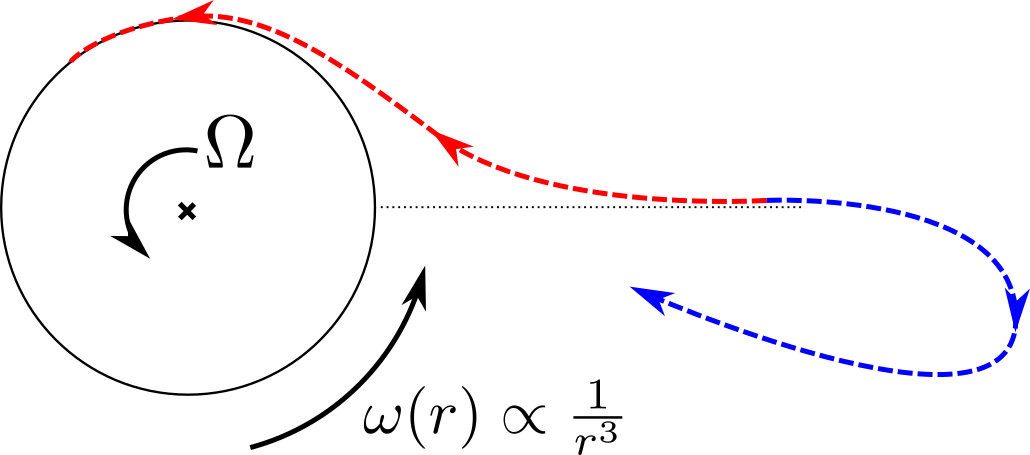
\includegraphics[scale=0.7]{{./images/frame-dragging.png}}
	\captionof{figure}{Frame-dragging effect over a massive rotating object on a free-falling body (red) and on a body that tries to move away from it (blue). Frame-dragging induces a force similar to the Coriolis--effect by \q{dragging} the compass of intertia in the direction of the star's rotation. Bodies falling towards the star's center are deflected in the direction of the rotation, while bodies moving away from it are deflected in the opposite direction.}
\end{figure}

\end{frame}